\vspace{2cm}
\noindent In this chapter the results of various simulations utilising the OxDNA based
rotaxane model are presented. The aim of this computational analysis is to shed light on
the entropic effects which play a central role in the nanopiston's operating cycle. By
extension, the thermodynamic transitions providing the free energy governing its
operation are studied.\\\\
To better understand the entropic interactions between the DNA rotaxane and the nanopore
a specially engineered rotaxane variant is studied. This other class of rotaxane is
called the mixed rotaxane, composing of different ds- and ssDNA fractions in an attempt
to isolate the influence of entropic interactions. Having explored the effects of the
entropic contributions, next the conformational fluctuations of the nanopiston are
simulated and analysed. Lastly, an attempt is made to simulate the thermodynamic
transitions driving the piston cycle. These particular simulations are made possible
by the use of a forward flux sampling algorithm.

\newpage

\section{Mixed Rotaxane}

Having identified the entropic interactions as key component of the nanopiston cycle,
studying them is an important but challenging task. The problem arises when we aim to
specify the entropic contributions to the conformal fluctuations of the rotaxane. The
main factor complicating this analysis is the multiplicity of the interactions acting
upon the nanopiston.\\

% Studying solely the contributions of entropic interactions in the conformal
% fluctuations  of the rotaxane is challenging task. The main factor complicating this
% analysis is the  multiplicity of the interactions acting upon the nanopiston.\\

The first category of forces is composed of the external forces arising from the
potential difference applied over the membrane. This potential difference induces an
electric field both outside and inside of the nanopore, influencing the movement of
molecules in these regions. The most significant contributions can be identified as the
electrophoretic and electro-osmotic forces acting upon the rotaxane. The second class of
forces is composed of the intrinsic forces. These forces do not arise from the
electric field, but rather originate from the direct interactions between the rotaxane
and the nanopore itself. Under this category fall the electrostatic, steric and entropic
forces, limiting the conformational freedom of the piston.



% Since both the DNA polymer and the ClyA nanopore have a net negative
% charge, the first intrinsic force can be identified as the electrostatic interaction
% between these two components of the piston. At short distances however this electrostatic
% force is dominated by the repulsive component of van der Waals forces arising from
% overlapping of the atoms' electron clouds. This contribution is referred to as the steric
% force. Lastly the entropic force is also categorised as a intrinsic force, arising from
% the reduction in available configurational micro states of the rotaxane upon confinement
% in the pore. [.]

In order to study the role of entropy in the conformational fluctuations of
the nanopiston, these effects need to be isolated from the other contributions present in
the system. To achieve this Bayoumi et al.[.] devised a new variation of the rotaxane
called the mixed rotaxane. In this rotaxane variation the toehold is removed, resulting
in a thread composed of solely ds- and ssDNA. By varying the DNA composition of this
rotaxane the changes in entropic interactions can be analysed. More specifically, the
total length of the rotaxane was constant, i.e. the total number of nucleotides and
basepairs are fixed at 100, while the ssDNA part was varied from $0nt$ to $30 nt$ in
steps of $10nt$. The effects of these changes in composition were first studied using I-V
measurements in the range of $[-100mV, +100mV]$. During an I-V measurement a range of
voltages is applied over the lipid membrane and at each step in this voltage sweep the
current through the pore is measured. A detailed explanation of this method is described
in.[. bay] The results from these experiments are presented in Figure....

The mixed rotaxane composed entirely of dsDNA yields an almost linear I-V trace in the
measured voltage range. This result indicates a constant obstruction of the nanopore over
the entire voltage sweep. On the other hand, the mixed rotaxane composed of a $10nt$
ssDNA strand shows a drastically different I-V trace. Decreasing the voltage below
$-20mV$ results in current fluctuations between two distinct levels. A second transition
can be observed when the voltage is further decreased below $-70mV$. Here the measured
current becomes independent from the applied voltage, suggesting a partial blockage of
the current through the nanopore. These same characteristics can be identified in the I-V
trace of
the mixed rotaxane with a $20nt$ ssDNA strand. Remarkably, the voltage range
in which the current fluctuations are observed is moved to a more negative
voltage range from $-30mV$ to  $-85 mV$. When the fraction of ssDNA in the mixed rotaxane
is further increased to $30nt$, the characteristic blockage is no longer observed and the
linear I-V trace is recovered.

\begin{figure}[ht!]

  \begin{centering}
  \adjustbox{minipage=1.3em,valign=t}{\subcaption{}\label{sfig:testa}}%
  \begin{subfigure}[t]{\dimexpr.29\linewidth-1.3em\relax}
  \centering
  \vspace{0.35cm}
  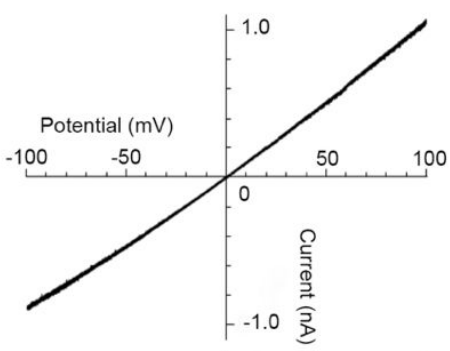
\includegraphics[width=1.05\linewidth,valign=t]{Figures/IV-100.png}
  \end{subfigure}%
  \adjustbox{minipage=1.3em,valign=t}{\subcaption{}\label{sfig:testb}}%
  \begin{subfigure}[t]{\dimexpr.5\linewidth-1.3em\relax}
  \centering
  \hspace{-0.2cm}
  \vspace{0.1cm}
  \includegraphics[width=0.95\linewidth,valign=t]{Figures/MR-100.png}
  \end{subfigure}%
  \adjustbox{minipage=1.3em,valign=t}{\subcaption{}\label{sfig:testc}}%
  \begin{subfigure}[t]{\dimexpr.21\linewidth-1.3em\relax}
  \centering
  \vspace{0.3cm}
  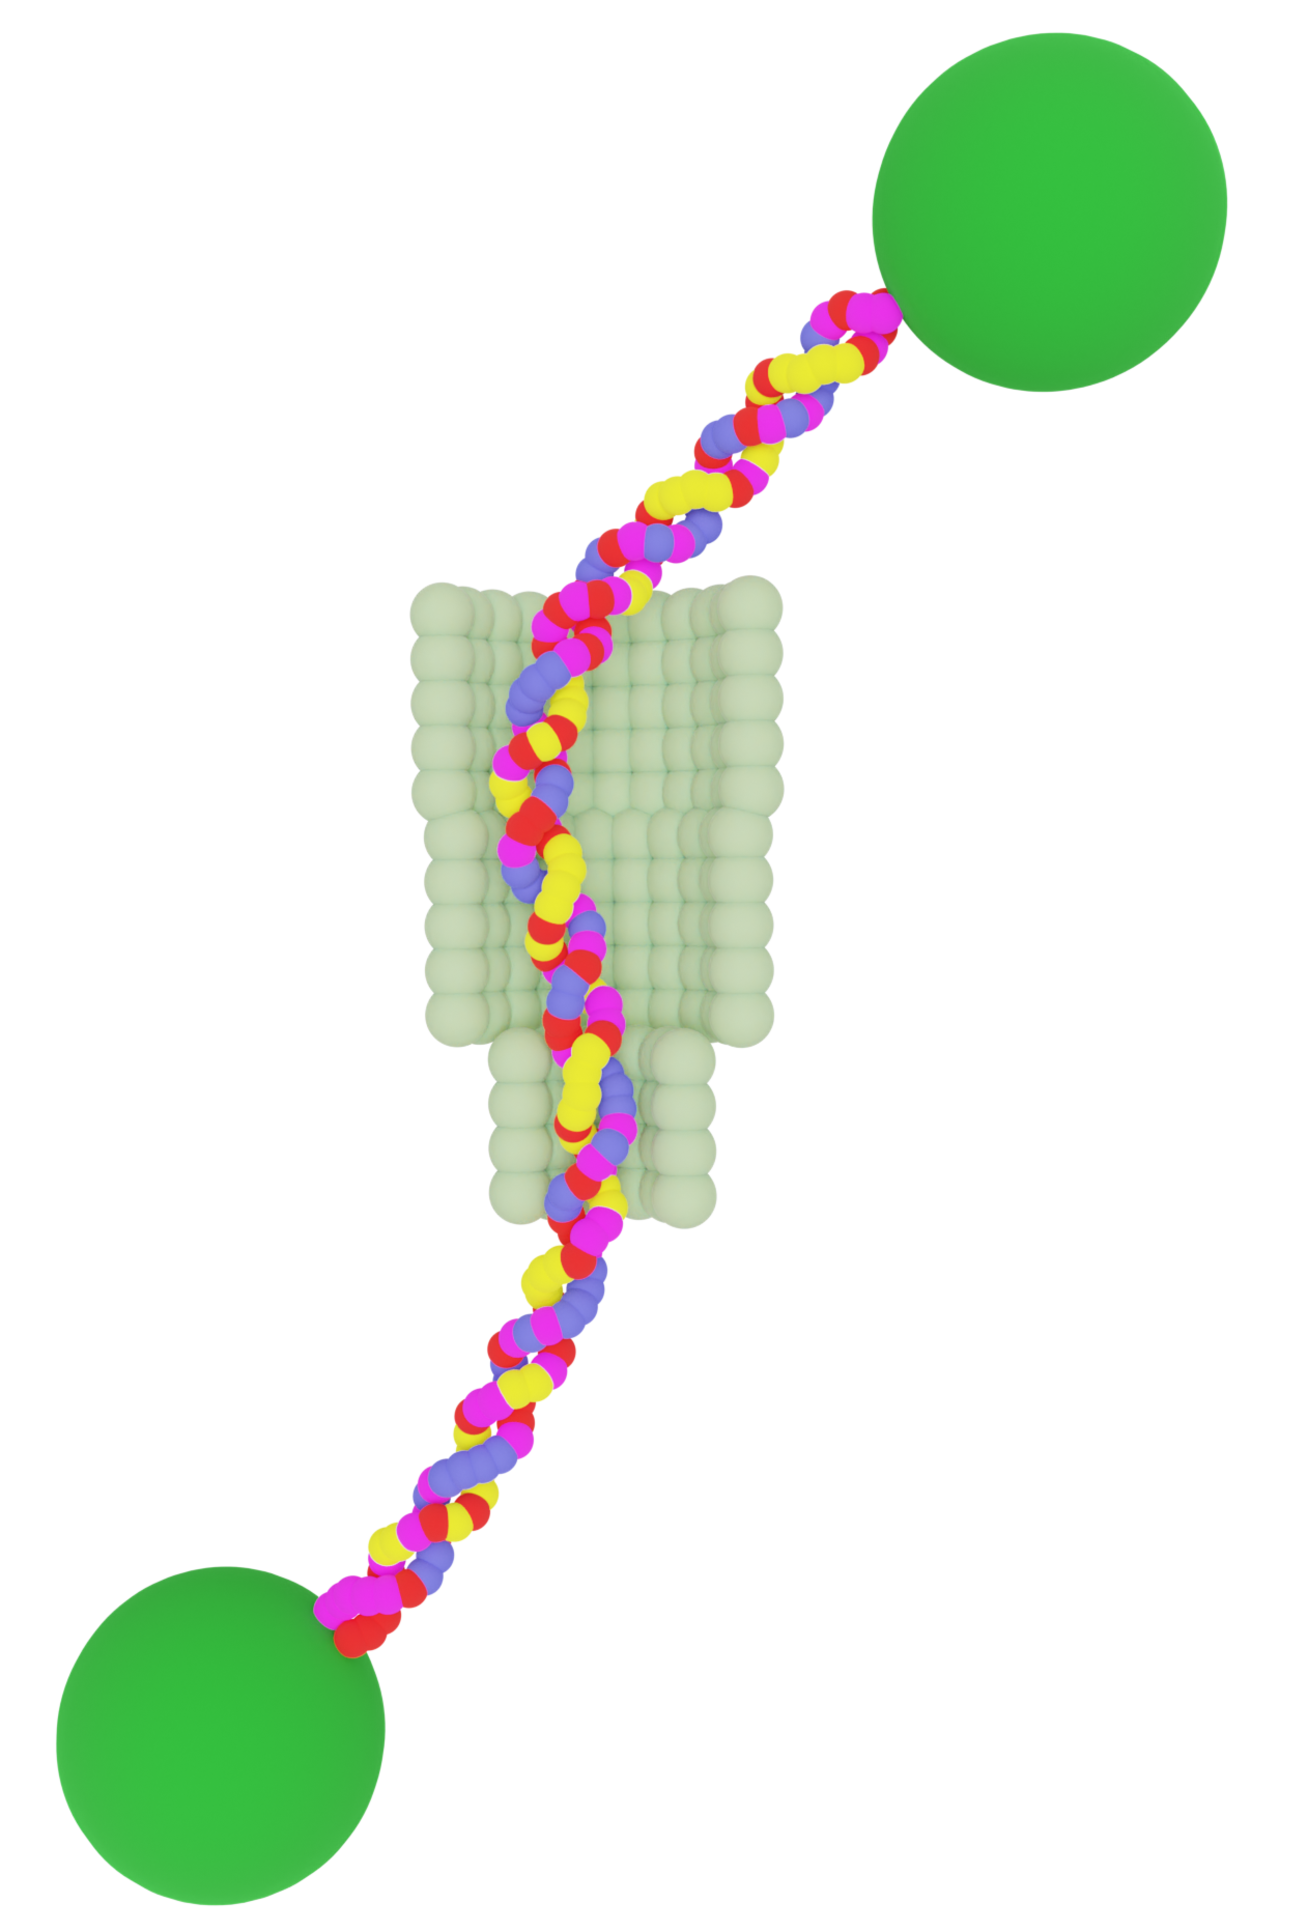
\includegraphics[width=0.8\linewidth,valign=t]{Figures/Rotaxane-100.png}
  \end{subfigure}
  \label{fig:test}
  \end{centering}

  \vspace{0.05cm}

  \begin{centering}
  \adjustbox{minipage=1.3em,valign=t}{}%
  \hspace{.35cm}
  \begin{subfigure}[t]{\dimexpr.3\linewidth-1.3em\relax}
  \centering
  \vspace{-0.1cm}
  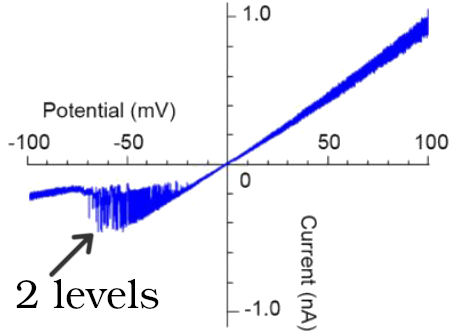
\includegraphics[width=1.05\linewidth,valign=t]{Figures/IV-90.png}
  \end{subfigure}%
  \adjustbox{minipage=1.3em,valign=t}{}%
  \hspace{.25cm}
  \vspace{-0.2cm}
  \begin{subfigure}[t]{\dimexpr.5\linewidth-1.3em\relax}
  \centering
  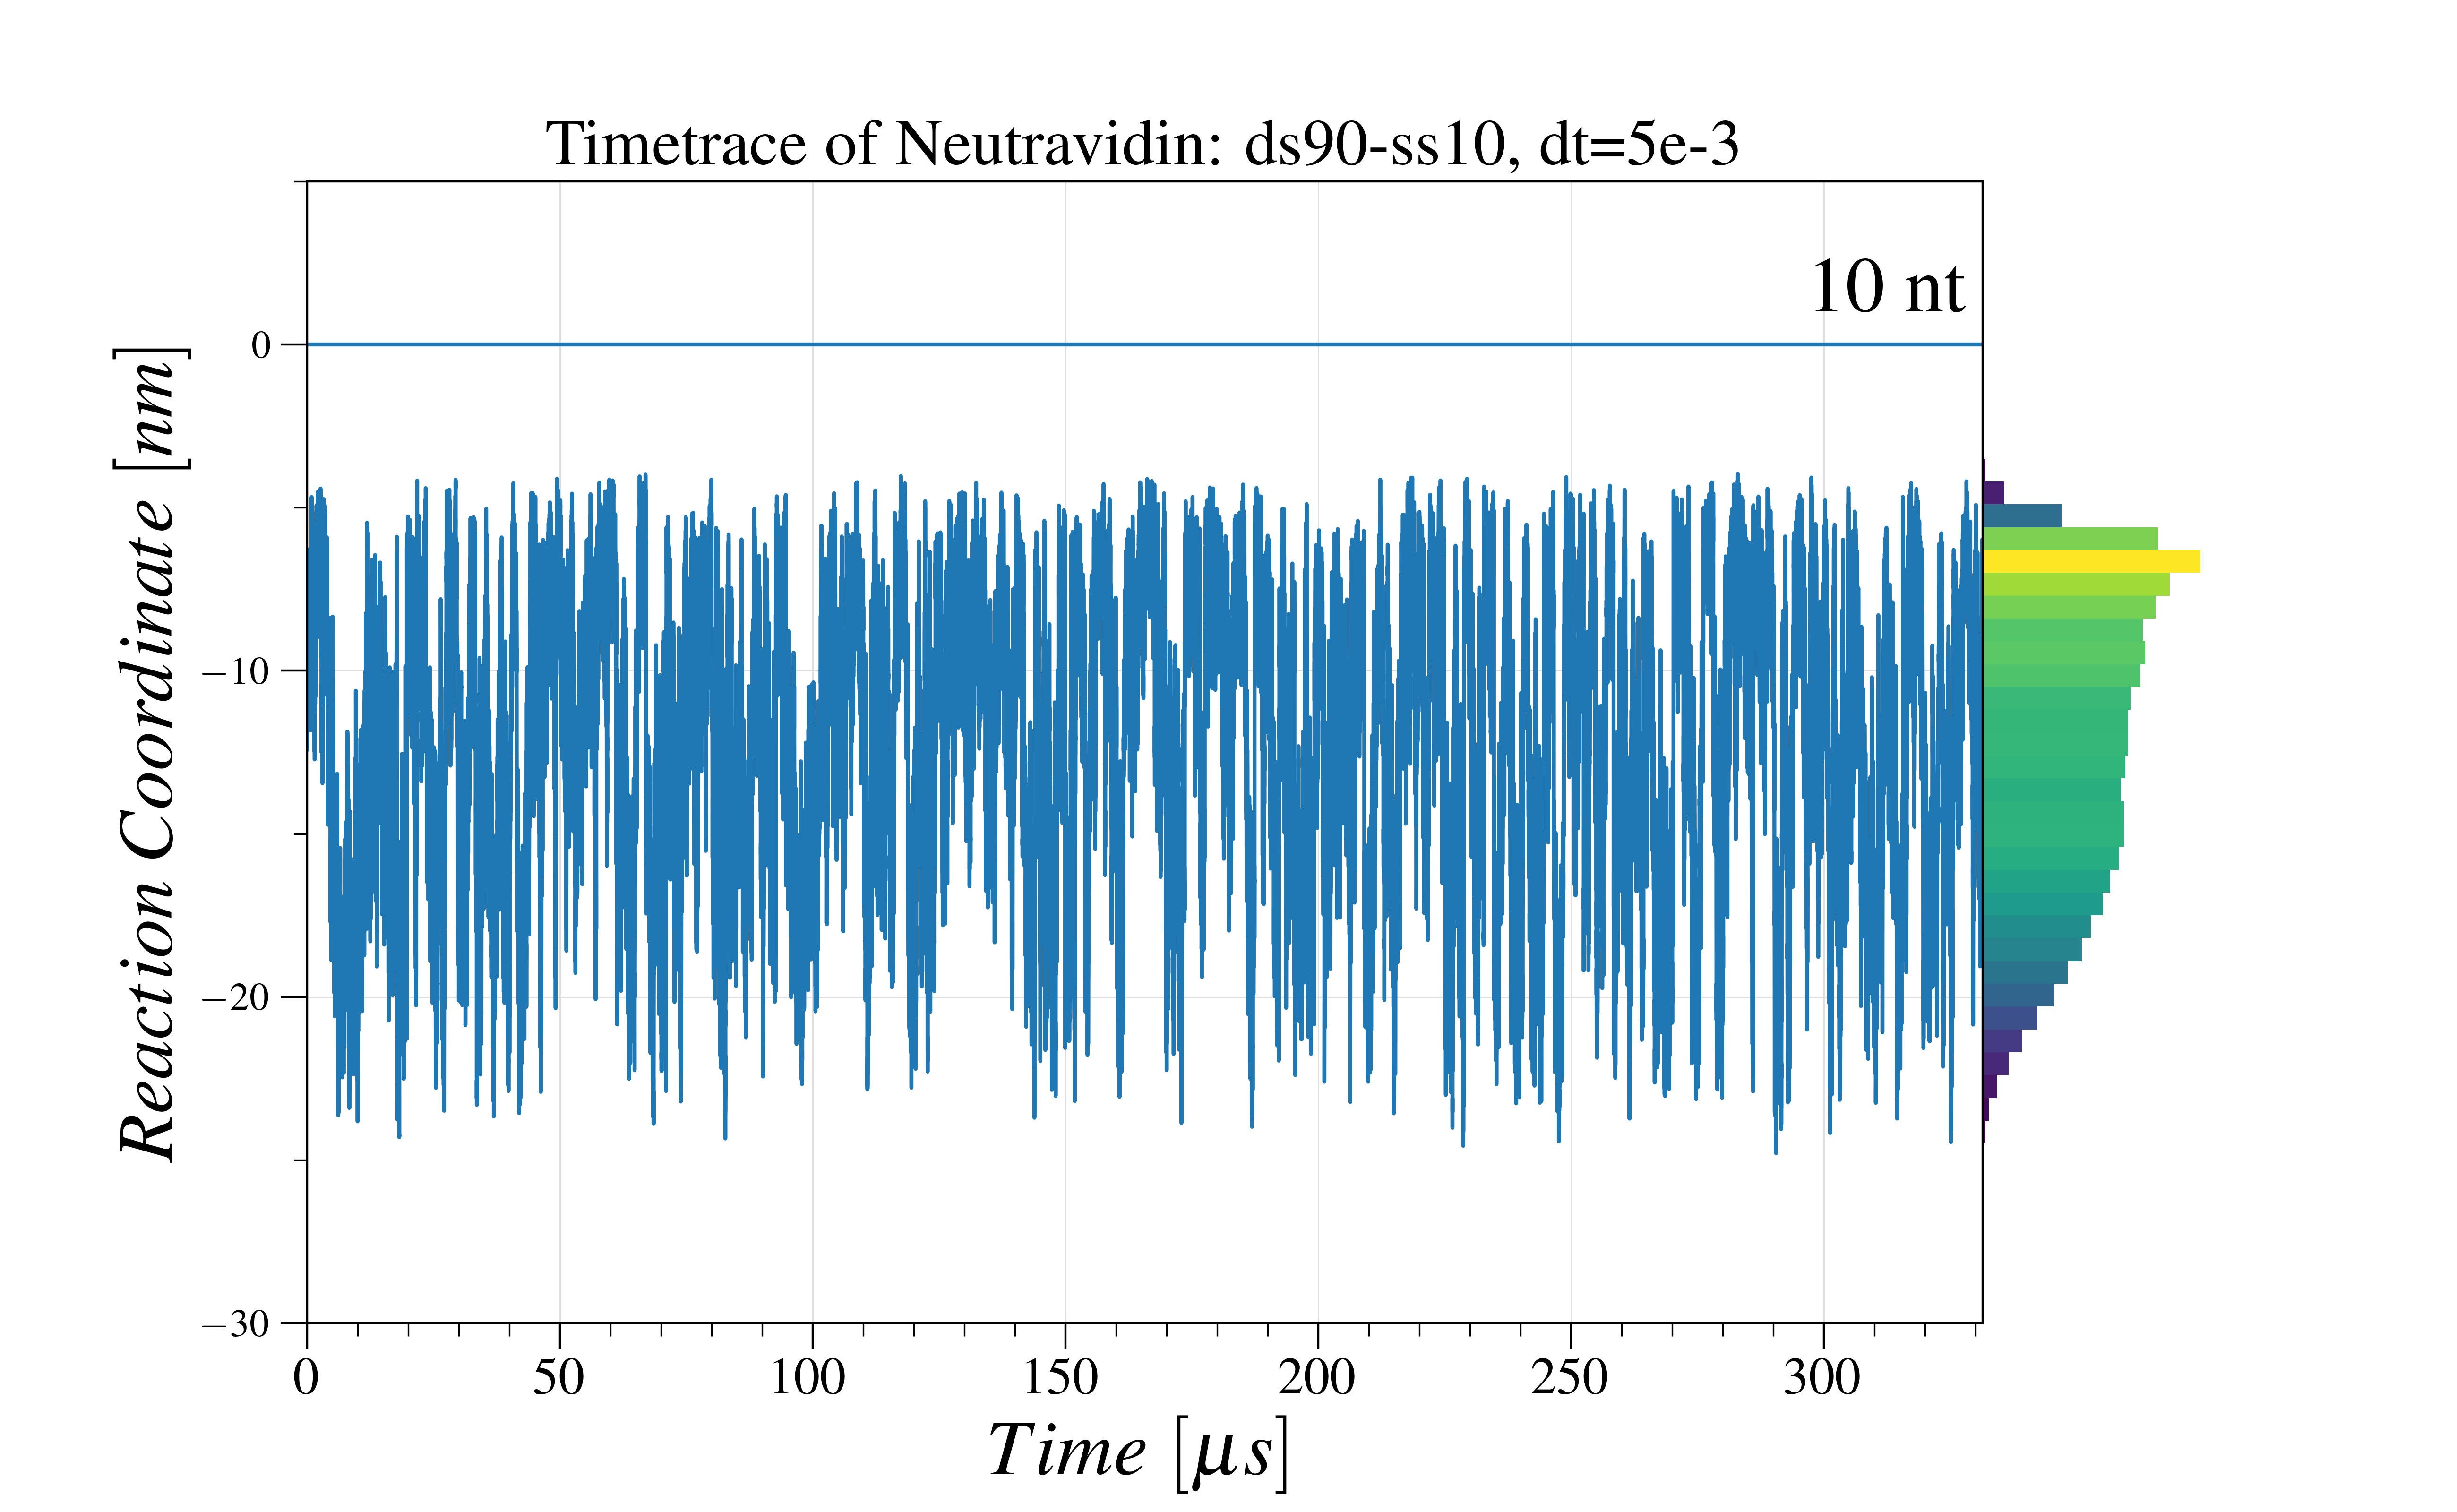
\includegraphics[width=.95\linewidth,valign=t]{Figures/MR-90.png}
  \end{subfigure}%
  \adjustbox{minipage=1.3em,valign=t}{}%
  \hspace{.3cm}
  \begin{subfigure}[t]{\dimexpr.21\linewidth-1.3em\relax}
  \centering
  \vspace{-0.5cm}
  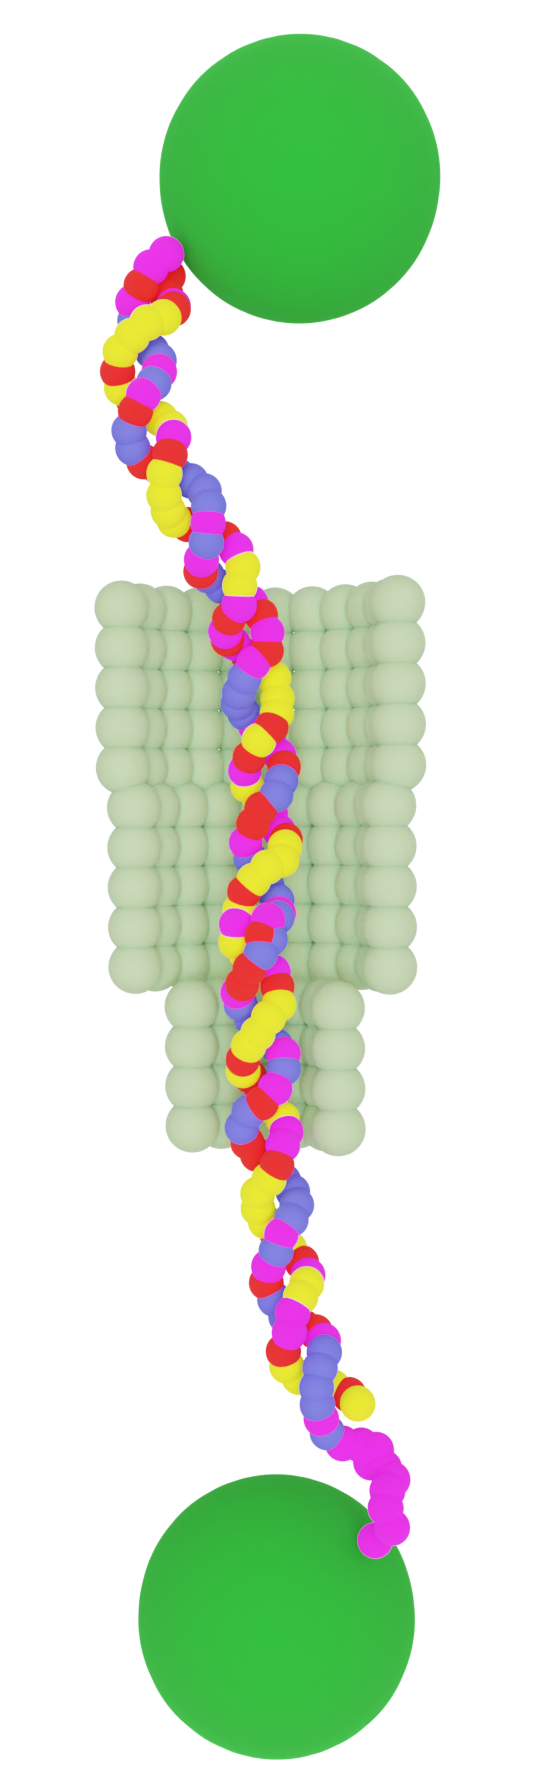
\includegraphics[width=.4\linewidth,valign=t]{Figures/Rotaxane-90.png}
  \end{subfigure}
  \label{fig:test}
  \end{centering}

  \vspace{.4cm}

  \begin{centering}
  \adjustbox{minipage=1.3em,valign=t}{}%
  \begin{subfigure}[t]{\dimexpr.3\linewidth-1.3em\relax}
  \centering
  \vspace{0.15cm}
  \hbox{\hspace{0.35cm}
  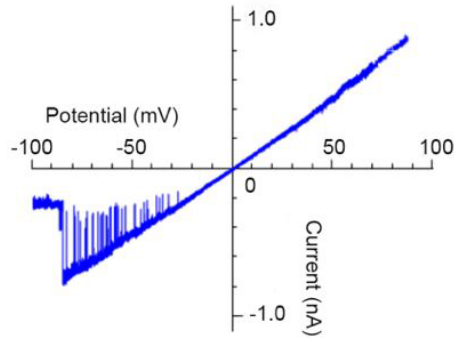
\includegraphics[width=1.05\linewidth,valign=t]{Figures/IV-80.png}}
  \end{subfigure}%
  \adjustbox{minipage=1.3em,valign=t}{}%
  \hspace{-0.5cm}
  \begin{subfigure}[t]{\dimexpr.5\linewidth-1.3em\relax}
  \centering
  \hbox{\hspace{0.56cm}
  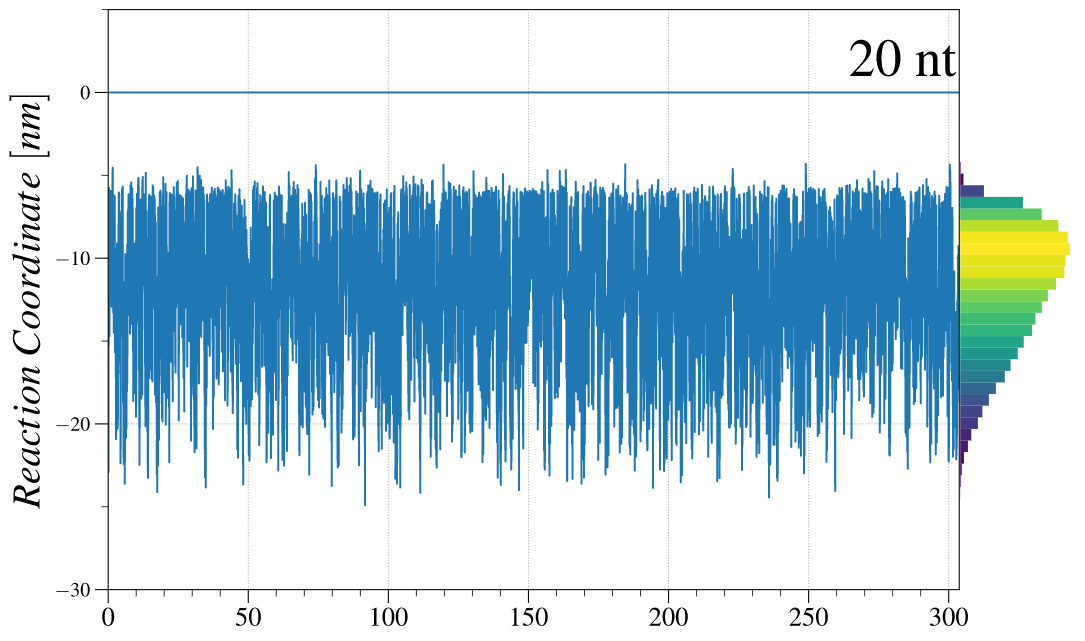
\includegraphics[width=.95\linewidth,valign=t]{Figures/MR-80.png}}
  \end{subfigure}%
  \adjustbox{minipage=1.3em,valign=t}{}%
  \hspace{.5cm}
  \begin{subfigure}[t]{\dimexpr.21\linewidth-1.3em\relax}
  \centering
  \vspace{-0.5cm}
  \hspace{-0.4cm}
  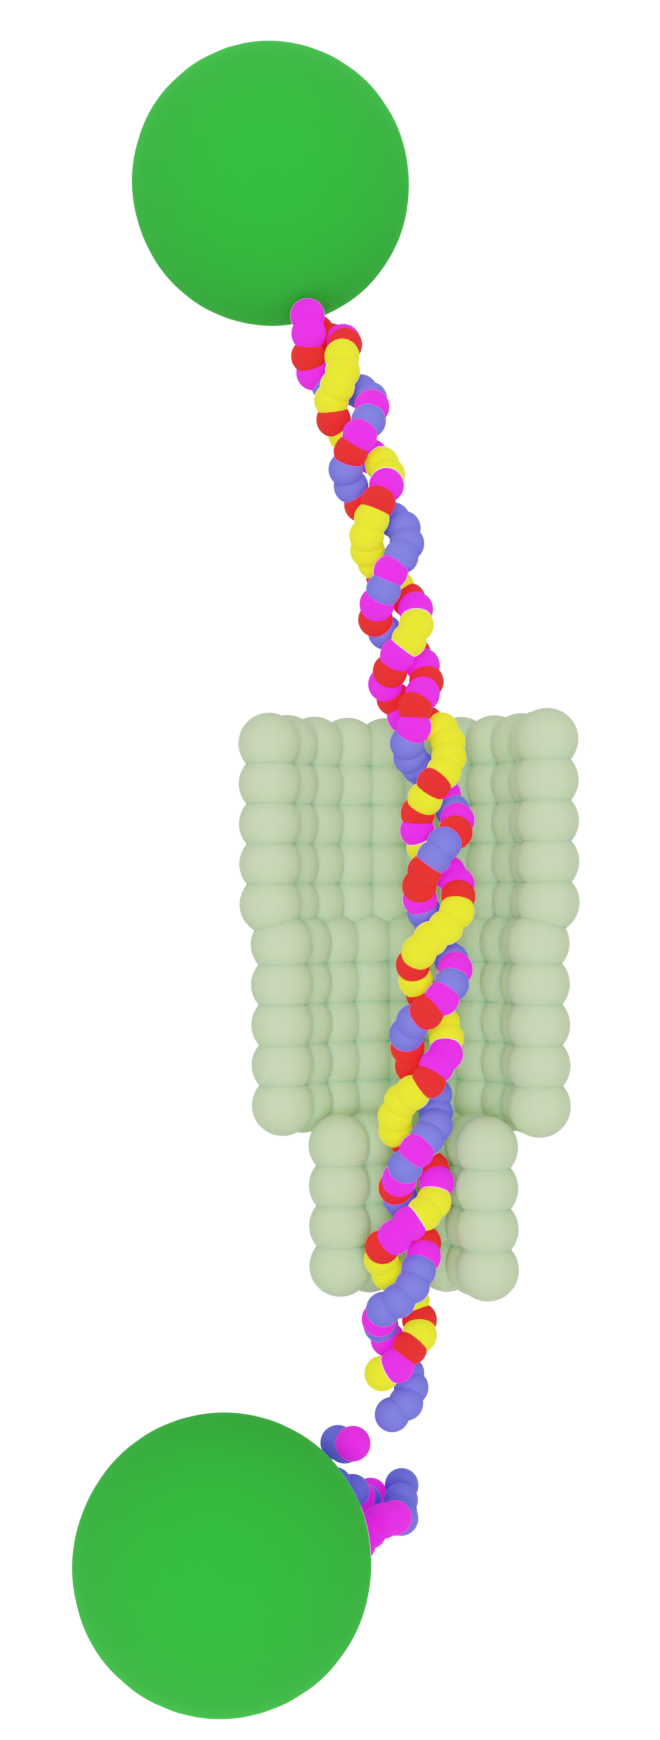
\includegraphics[width=.5\linewidth,valign=t]{Figures/Rotaxane-80.png}
  \end{subfigure}
  \label{fig:test}
  \end{centering}

  \vspace{.25cm}

  \begin{centering}
  \adjustbox{minipage=1.3em,valign=t}{}%
  \begin{subfigure}[t]{\dimexpr.3\linewidth-1.3em\relax}
  \centering
  \vspace{0.2cm}
  \hbox{\hspace{0.4cm}
  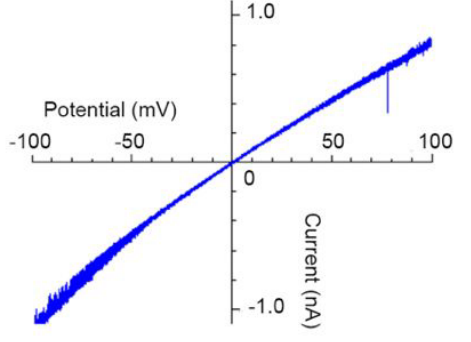
\includegraphics[width=1.05\linewidth,valign=t]{Figures/IV-70.png}}
  \end{subfigure}%
  \adjustbox{minipage=1.3em,valign=t}{}%
  \begin{subfigure}[t]{\dimexpr.5\linewidth-1.3em\relax}
  \centering
  \hbox{\hspace{0.15cm}
  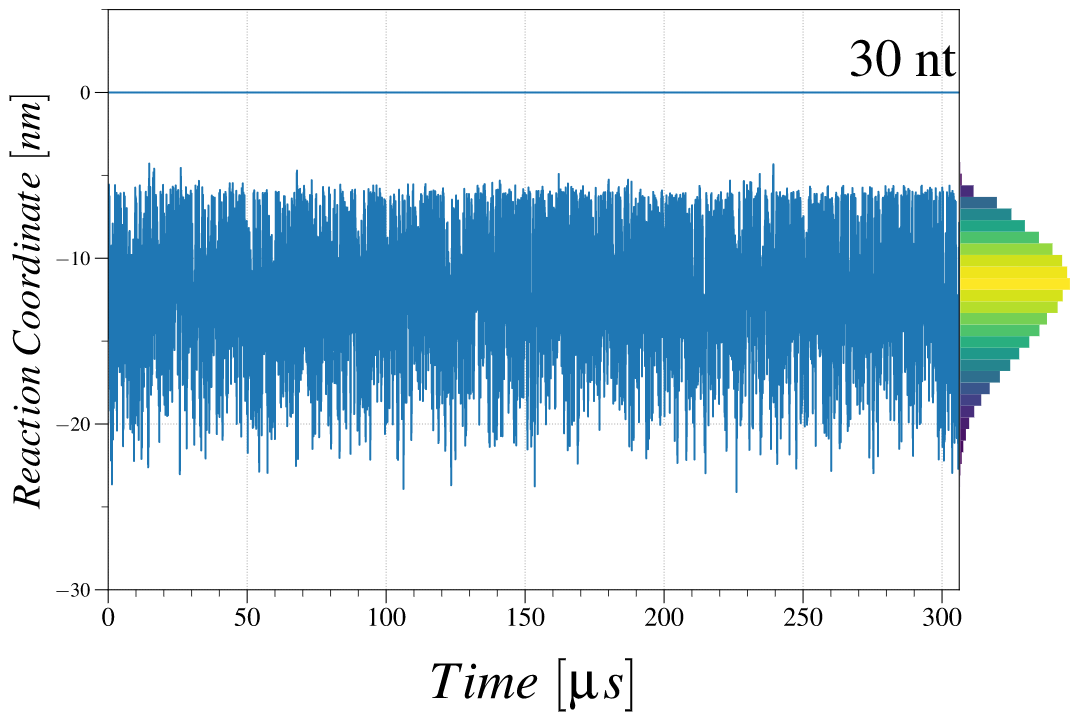
\includegraphics[width=.95\linewidth,valign=t]{Figures/MR-70.png}}
  \end{subfigure}%
  \adjustbox{minipage=1.3em,valign=t}{}%
  \hspace{0.5cm}
  \begin{subfigure}[t]{\dimexpr.21\linewidth-1.3em\relax}
  \centering
  \vspace{-0.6cm}
  
\includegraphics[width=.35\linewidth,valign=t]{Figures/Rotaxane-70.png}
  \end{subfigure}
  \label{fig:test}
  \end{centering}
  \caption{This is a figure.\vspace{2cm}}

\end{figure}

To interpret the observed characteristics in the I-V traces, molecular dynamics
simulation where performed of the mixed rotaxanes. The rotaxanes where simulated with no
bias, i.e. $0 mV$, to solely highlight the changes in the entropic effects. Quantifying
the conformational fluctuations of the rotaxane is done by tracing the trans-stopper
protein during the simulation using a reaction coordinate defined in our system. This
reaction coordinate, $X$, is determined as,
\begin{equation}
  X = \begin{cases}
        &z_0 + |\textbf{r} - \textbf{r}_{cis}|, \hspace{0.5cm} \textit{if on cis-side}\\
        &z, \hspace{2.5cm} \textit{if inside pore}\\
        &-|\textbf{r}|, \hspace{2.11cm} \textit{if on trans-side}
      \end{cases}
\end{equation}
Here the z-axis is aligned with the symmetry axis of the nanopore, placing the origin of
the coordinate system at center of the pore's trans-entrance. With respect to this
coordinate system, the center of pore's cis-entrance is located at $r_{cis} = (0,0,z_0)$.

In Figure ... the measured time trace of the $X$-coordinate is presented for each mixed
rotaxane type.  The horizontal line indicates the origin of the reaction coordinate,
representing the trans-entrance of the pore. On the right side of these graphs the $X$
histograms of the time traces are presented, indicating the positional distribution of
the trans-stopper during the simulations. It should be noted that the time traces are not
obtained from one continuous simulation, but rather aggregated from various independent
simulations performed in parallel, aiming to reduce the simulation time.

For the rotaxane fully composed of dsDNA, i.e. $0nt$, a uniform  $X$  histogram is found.
This result indicates free diffusion of the rotaxane within a bounded one dimensional
domain, namely the nanopore. In the case where $10nt$ and $20nt$ are substituted into the
composition of the rotaxane a peak is observed in the $X$ histogram. This peak indicates
a tendency of the trans-stopper to move towards the entrance of the nanopore. This
observation is in agreement with the previously discussed I-V curves, since the presence
of the stopper at the pore entrance partially blocks the current flow. This tendency
is driven by an entropic force arising from the smaller ssDNA strand, being more easily
captured in the constriction of the pore compared to the large dsDNA strand.


Next, we observe that increasing the length of the ssDNA part of the mixed rotaxane
gradually shifts the histogram's peak further away from the pore entrance. Confining a
portion of the freely fluctuating ssDNA strand inside of the pore,
drastically reduces the number of available configurational microstates and thereby also
its entropy. This change in entropy induces an opposing entropic force.
An equilibrium configuration is found, when both the large dsDNA is kept outside of the
constriction, while allowing a maximal length of ssDNA strand to freely fluctuate outside
of the pore. These combined effects shift the peak of the distribution further away from
the pore entrance as the number of nucleotides is increased. An ever larger
electrophoretic force is required to sustain full pore blockage, which is why no blockage
is observed in the experiment's voltage range. The results found in these simulations are
in accordance with the corresponding simulations performed by Bayoumi et al.[.], using
the bead-and-spring model.

As the final part in our analysis of the mixed rotaxanes, the confined diffusion of the
$0nt$ mixed rotaxane is studied. The uniform distribution of the $X$ histogram suggests
that the rotaxane vertically fluctuates inside of the pore like a rigid rod. To study
this diffusive behaviour, the mean square displacements(MSD) of the
trans-stopper is determined within a range of time intervals.\footnote{reference
tidynamics by Pierre de Buyl} Calculating the MSD is done by utilising a rolling-window
analysis on the measured time trace. The MSD is an important quantity used to
characterise diffusive processes, since it allows us to verify whether an external force
influences the motion. From analytical calculations, presented in appendix A, we find
that one dimensional confined diffusion can be described up to the second order as,
\begin{equation*}
\langle \Delta x \rangle = \frac{L^2}{6} - \frac{96}{\pi^4} e^{-\frac{D \pi^2t
}{L^2}},
\end{equation*}
here $L$ is the length of the confined region, i.e. the hight of the pore, and $D$ the
diffusion constant of the particle. This model was fitted to our simulations, for which
the result is presented in Figure... From this we can conclude the $0nt$ mixed rotaxane
can be well described using the simple model of one dimensional confined diffusion,
confirming our postulation. This model predicts the diffusion coefficient of the mixed
rotaxane as, $69.08 \pm 0.02 \mu s^{-1}$, giving us an idea of the speed of the
rotaxane dynamics.

\begin{figure}[ht!]
\begin{center}
  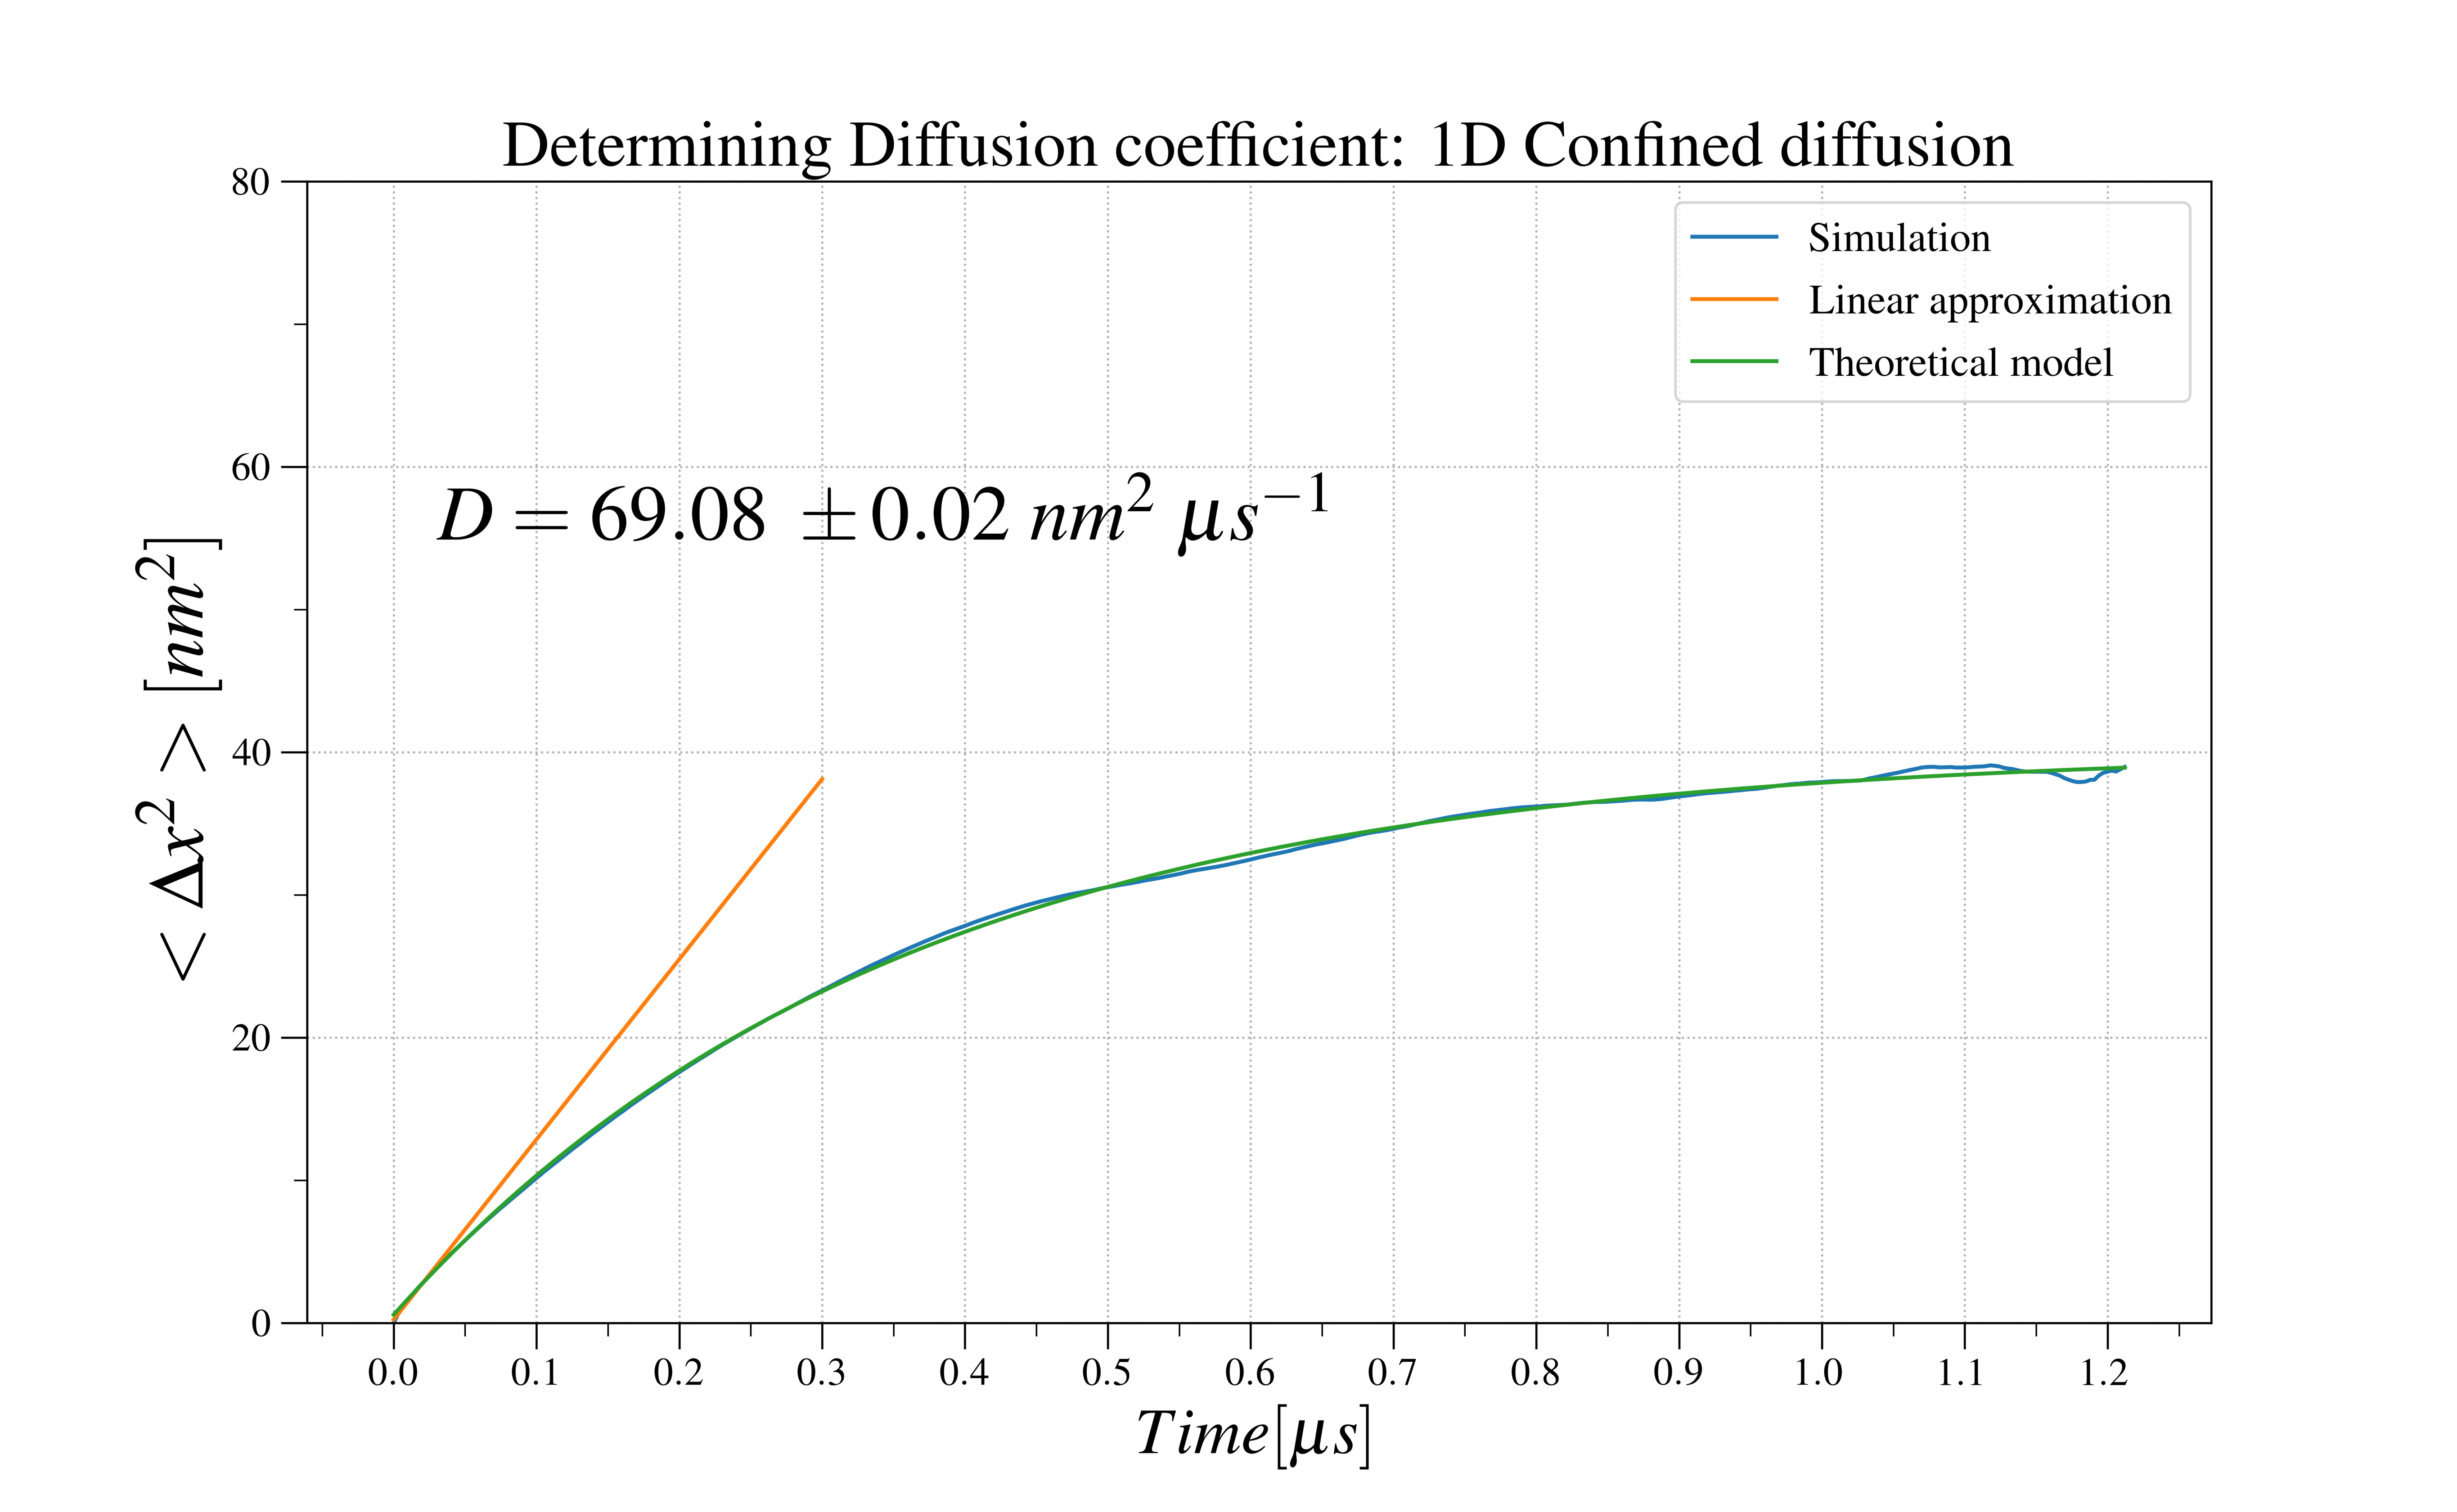
\includegraphics[width=\textwidth]{Figures/MR-100-diff.png}
  \caption{write caption}
\end{center}
\end{figure}
